



\begin{frame}{\citetitle{Avatar3d_Echartea_2021} \footnotemark (1)}
%\begin{block}{Aplicación Movil para Concientizar a Niños Acerca del Cuidado del Peso (1)} 
	\begin{itemize}
\item Se requieren herramientas que apoyen en la concientización de problemas médicos graves (Obesidad)
\item Se integra una aplicación móvil que muestre un avatar tridimensional cuyo peso, estatura y edad sea configurable con por usuario
\item Es posible configurar el numero de comidas y el tipo de ejercicio de la simulación
\item Al finalizar la simulación, la aplicación mostrará el antes o despues basado en en los IMCs y los parametros del avatar. 
\item Herramientas utilizadas
	\begin{itemize}
		\item Unity
		\item MakeHuman 
	\end{itemize}
	\end{itemize}
%\end{block} 
\footnotetext[1]{\fullcite{Avatar3d_Echartea_2021}}
\setcounter{footnote}{0}
\end{frame}

\begin{frame}{\citetitle{Avatar3d_Echartea_2021} (2)}
%\begin{block}{Simulación de modelo de diabetes en un dispositivo móvil (2)} 
\begin{center}
     \begin{tabular}{ccc}
         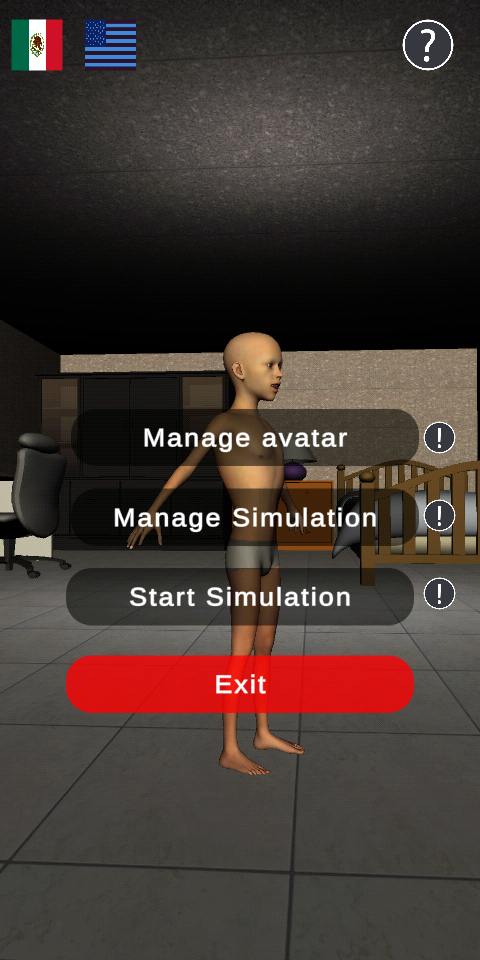
\includegraphics[width=0.25\textwidth]{Figs/Echartea1}&
         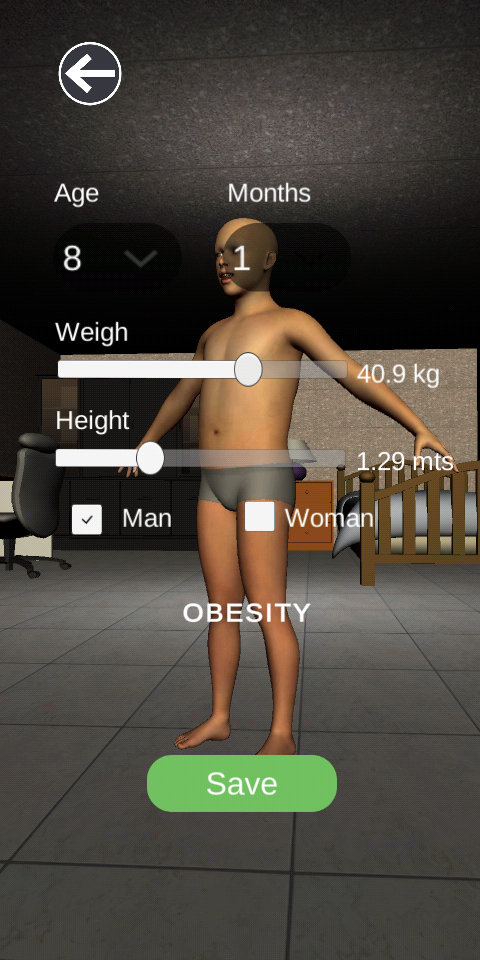
\includegraphics[width=0.25\textwidth]{Figs/Echartea2}&
         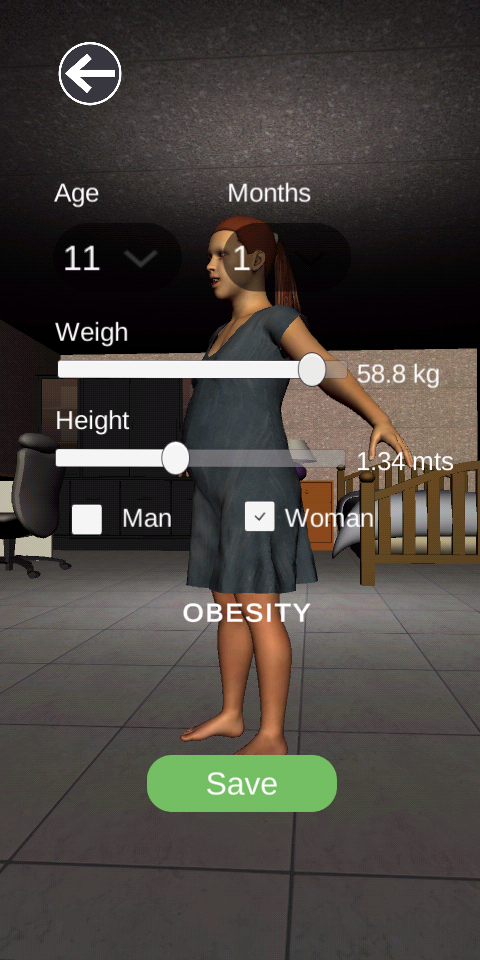
\includegraphics[width=0.25\textwidth]{Figs/Echartea3}\\
          \end{tabular}
\end{center}
%\end{block} 
\end{frame}

%\begin{frame}{Proyectos de Investigación}
\begin{frame}{\citetitle{Avatar3d_Echartea_2021} (3)}
%\begin{block}{Simulación de modelo de diabetes en un dispositivo móvil (2)} 
\begin{center}
     \begin{tabular}{cc}
         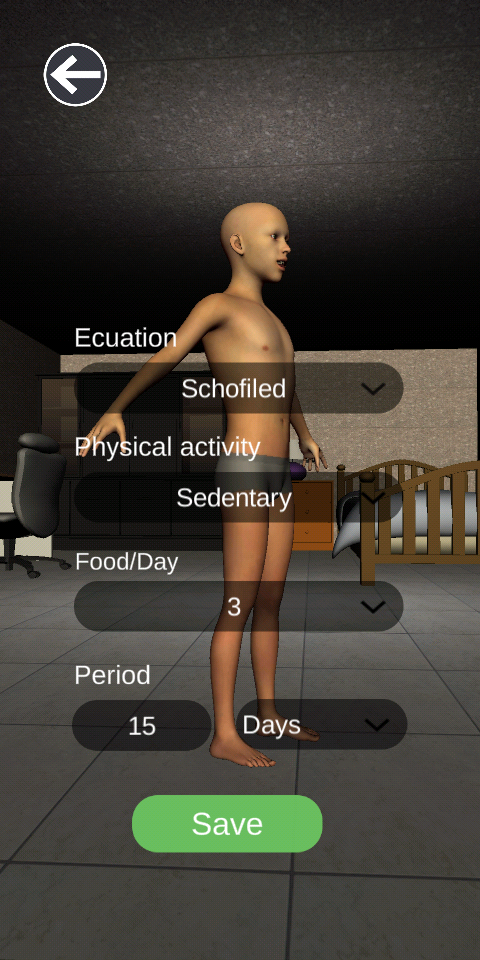
\includegraphics[width=0.25\textwidth]{Figs/Echartea4}&
         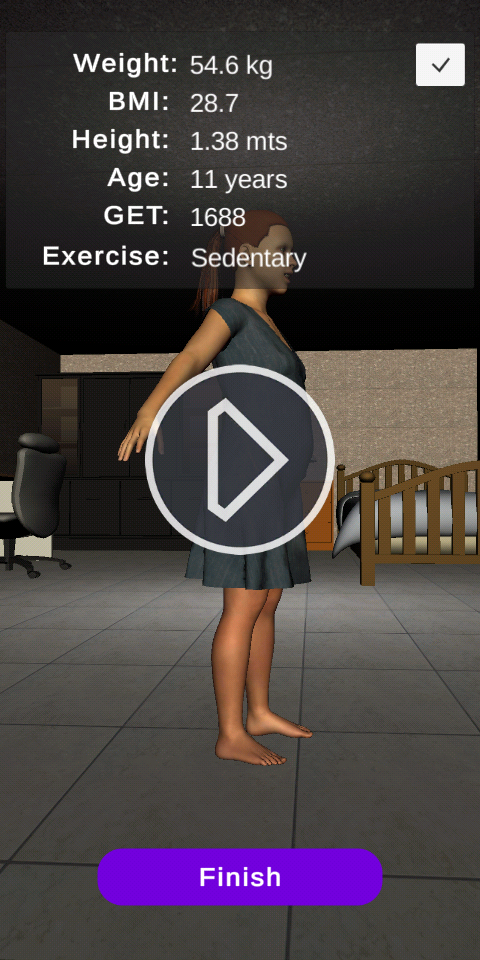
\includegraphics[width=0.25\textwidth]{Figs/Echartea5}
          \end{tabular}
\end{center}
%\end{block} 
\end{frame}

